\subsection*{Chaos Shrine}
As the party reaches the grasslands at the edge of the dark forest, they can see the menacing Chaos Shrine in the distance.
As they move closer, they notice that the shine has mostly been claimed by nature, as its walls are damaged and overgrown and the foundation has begun to sink into the ground.
An unnatural serenity surrounds the shrine with no other living being in sight and the only entrance is a set of brittle stairs that lead down into darkness. 
After descending the stairs, the party arrives at the south of the map shown below and can barely see in the dark.
The way north is blocked from rubble that is a product of pillars and large rocks which have broken off from the ceiling.
Upon closer inspection, the party realizes that this blockade has been created purposefully.
\vspace{0.1cm}
\tcbox[left=1pt,top=1pt,right=1pt,bottom=1pt, boxsep=-1pt, colframe=accent, sharp corners]{
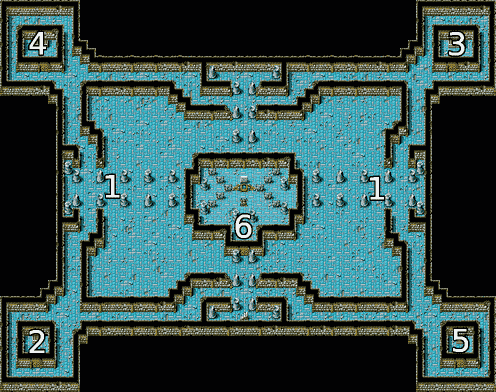
\includegraphics[width=0.98\columnwidth]{./art/maps/shrine.png}}

\subsubsection*{1. Traps}
Both marked locations contain a magical trap on the ground that has been placed by Garland to alert him and  impede intruders.
A character that is actively looking for traps or taking similar precautions notices it by passing a DC~7 check. 
The trap explodes when stepped, dealing 2d \hyperlink{type}{fire} damage to everyone within 1u of its center. 

\subsubsection*{2. Mimic}
Inside this room is a single large chest that once touched reveals itself to be a vicious Mimic.
A character can notice that something is wrong with the chest beforehand by passing a DC~9 check.
If they fail to do so, the Mimic automatically gets the best possible result for his initiative check in the ensuing battle.
\vfill
\monster{Mimic}{2}{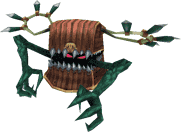
\includegraphics[width=0.25\textwidth]{./art/monsters/mimic.png}}
{
	HP: & \hfill 20 & MP: & \hfill 0\\
	STR: & \hfill 2 & DEF: & \hfill 0 \\
	MAG: & \hfill 0 & RES: & \hfill 0 \\
	AGI: & \hfill 2 & Size: & \hfill M\\
}
{
	\textbf{Bite}: 1d DMG \hfill \textbf{Drops:} 200 Gil	
}

\subsubsection*{3. Healing Spring}
The heavy door of this room is locked and can be broken or lockpicked, by passing a check whose DC can vary from 6 to 9 depending on the character's expertise.
Inside the room, the party finds a large chalice that stands on a stone pedestal and is filled with what seems to be water.
Upon closer inspection, a character can understand that the liquid is of magical nature and a character that drinks it, fully recovers his HP and MP immediately.
However, the chalice itself has no magical properties and contains only 5 portions of the healing water.

\subsubsection*{4. Chests}
This room contains 2 chests, one can be opened easily and contains 3 \hyperlink{item}{Potions} and a \hyperlink{item}{Phoenix Down}.
The other one contains \textbf{Sarah's Lute} and can only be lockpicked by passing a check where the DC varies between 7 and 10 depending on the character's expertise.
It can also be opened with a key that Garland carries with himself, but the chest is too robust to be broken through force.

\subsubsection*{5. Secret Door}
This room is empty except for a large stone tablet on the left wall with multiple different symbols on it.
Upon closer inspection, the party can understand that the symbols describe a short music piece. 
The wall next to it contains a secret door which is revealed by playing the piece on Sarah's Lute, which only Sarah herself should able to perform properly enough.
The secret door leads into a small room with a stone pedestal which has the following item on it:  
\vspace{0.3cm}
\accessory{Accessories}{acc.png}{
	\hline Angel Ring & 2000 Gil & When you suffer \hyperlink{status}{KO} while wearing this ring, you can activate its effect to immediately get revived with 1 HP. The ring is destroyed after using this effect. \\
} 
%\pagebreak
\subsubsection*{6. Garland}
"Hmph. The king's lapdogs. Do you have any idea who you're messing with?"
\indent -- Garland \\\\ 
At the center of the temple, the party finally confronts Garland.
Sarah is also in this room, locked in a cage that stands in its corner. 
Garland is a tall, well-built man in full heavy armor wearing a purple cape and carrying a sword.
He is very arrogant and believes that he deserves to rule Cornelia, because he is the strongest warrior in the kingdom.
Garland has studied the dark secrets of the Chaos Shrine since his arrival to expand his power.
He sees the party as just another annoyance standing in the way of his grand plans.

\subsubsection*{Final Battle}
"You really think you have what it takes to cross swords with ME? Very well..." \\
\indent -- Garland \\\\ 
Garland draws his weapon to commence the fight and he also summons multiple bats to aid him, one for each party member.
During the battle, he focuses on his positioning to pick off lone party members while he avoids getting outnumbered himself.
He prefers to stand behind his minions to use his ranged abilities at first and tries to finish off enemies that have been weakened later on.  
In the original story, Garland uses a magical artifact to escape after being defeated and goes on to become the main antagonist of the game.
If you want to continue the adventure differently, he may also die at hand of the adventurers or you can let the players decide his fate.
After being freed from her prison, Sarah is understandably still very scared and traumatized.
She thanks the party for rescuing her and asks them to find her precious lute, which Garland has taken.
The party can refuse her request to quickly return to Cornelia, which Sarah will understand but not be happy about.

\vfill
\monster{Murciélago}{1}{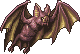
\includegraphics[width=0.18\textwidth]{./art/monsters/bat.png}}
{
 PV: & \hfill 6 & PM: & \hfill 0\\
 FUE: & \hfill 0 & DEF: & \hfill 0 \\
 MAG: & \hfill 0 & RES: & \hfill 2 \\
 AGI: & \hfill 4 & Tamaño: & \hfill P\\
}
{
 \textbf{Dientes}: 1d de daño \hfill \textbf{Botín:} 100 Gil 
 
 \mpassive{Absorber}{Por cada \hyperlink{action}{Ataque} exitoso, recuperas 1d de PV.} 
}
\vfill
\monster{Garland}{3}{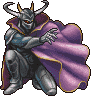
\includegraphics[width=0.18\textwidth]{./art/monsters/garland.png}}
{
 PV: & \hfill 40 & PM: & \hfill 30\\
 FUE: & \hfill 3 & DEF: & \hfill 1 \\
 MAG: & \hfill 1 & RES: & \hfill 1 \\
 AGI: & \hfill 2 & Tamaño: & \hfill M\\
}
{
 \textbf{Espada Larga}: 1d de daño \hfill \textbf{Botín}: 1000 Gil, Llave 
 
 \mspell{Absorber}{8}{1t}{Único}{3u}{ Reduces 1d de los PV del objetivo y recuperas tus PV por el mismo valor.}{} \mspell{Silencio}{6}{1t}{Único}{3u}{El objetivo hace una tirada con DC 8. Si falla, sufre \hyperlink{status}{Silencio} por 3 turnos.}{\silence}
 \mreaction{Parada}{Cuando falles al intentar esquivar un \hyperlink{action}{Ataque}, Puedes hacer una tirada con DC~8. Si tienes éxito, el daño que recibes se reduce a la mitad.}
}

\pagebreak

\subsection*{Epilogue}
"You... you've come to rescue me? I don't know how I can ever thank you..." \\ 
\indent -- Sarah \\\\ 
After rescuing Sarah, the party has to return her safely to Cornelia and therefore, they have to travel back the long path they came from.
The journey should be uneventful for the most part, but you can feel free add a few surprises of your own.
Sarah is a young princess with turquoise hair like her mother and wears a gold colored dress as well as a golden pendant with red jewels.
She is polite but also very quiet and absent, because she is suffering from the physical and mental scars of the kidnapping.
Sarah is not capable of looking after herself, so she needs the adventurers' assistance and guidance during the journey.
While travelling, she often asks about the state of Cornelia and her family as she blames herself for what has happened.

\subsubsection*{Arrival}
"Thank you for returning my daughter to my side." \\ 
\indent -- King of Cornelia \\\\ 
When entering Cornelia with the princess at their side, the adventurers are hailed as heroes by the townspeople and guards.
Accordingly, they are recognized by everyone in the town as such from now on. 
The inhabitants of the castle are surprised when meeting the party, as they had already given up hope of ever seeing the princess again.
The king is very grateful to the adventurers and orders his servants to prepare a huge banquet in their honor on the evening of their arrival.
The party is rewarded with a \textbf{Level Up} after safely bringing the princess home.
Furthermore, the king offers them very generous rewards for rescuing his daughter as he had promised.
In the original story, the king commands his men to rebuild an old broken bridge, that leads to another large continent for the adventurers to explore.
Depending on how you want to continue the game, his gift should be something that greatly aids the party on their upcoming adventures.
He could for example gift them a ship that allows them to reach new lands or he could gift them a house in Cornelia if the city is still going to be relevant in the following.

\subsubsection*{Outlook}
By rescuing princess Sarah and defeating Garland, the party has grown together and developed their individual skills.
Even though they still have a lot to learn, they have proven themselves to be capable adventurers that can stand up against the evil in the world.
From here, you can continue the adventure by building on the presented content and creating your own locations, characters and challenges.
Before departing, the party may choose to spend some more time in Cornelia to rest and stock up on items and equipment.
